\section{Power Amplifier}

\subsection{Receiver Switch}
First, the receiver switch was built in order to protect the Rx circuitry when
the transmitter is active. The schematic of the filter is shown in
Figure~\ref{fig:RxSwitch}.

\begin{figure}[h!]
  \centering
  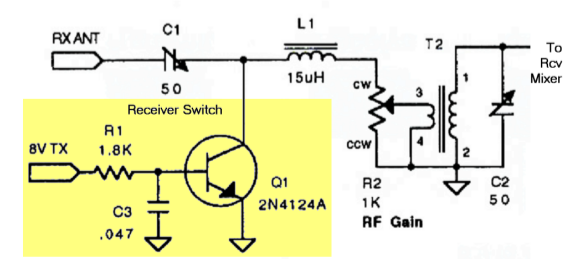
\includegraphics[scale=0.8]{./img/RxSwitch.png}
  \label{fig:RxSwitch}
  \caption{Receiver Switch}
\end{figure}

After the installation of the switching circuitry, the power amplifier was then
build according to the schematic shown in Figure~\ref{fig:powamp}.

\begin{figure}[h!]
  \centering
  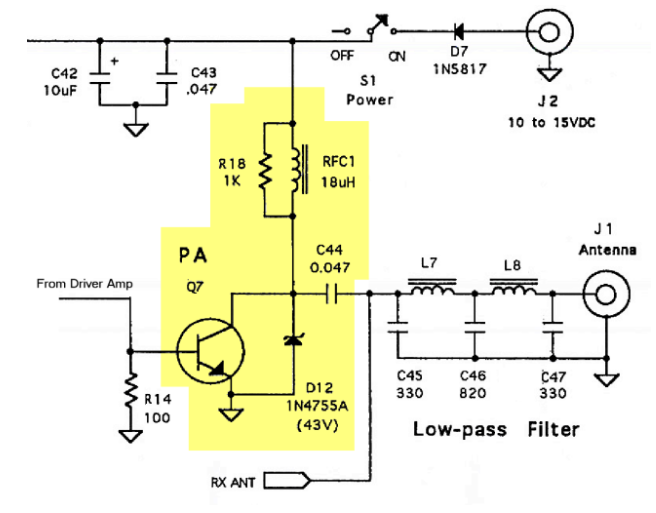
\includegraphics[scale=0.7]{./img/powamp.png}
  \label{fig:powamp}
  \caption{Power Amplifier}
\end{figure}

\subsection{Measurements}
In order to prevent cooking the oscilloscope, a 30dB attenuator was connected
between the antenna terminal and
%Ranging from 5V to 30V

\begin{tabular}{|c|c|c|c|c|}
  \hline
  Output Voltage $V_0$ & Output Power $P$  & Supply Power $P_0$  & Efficiency
  $\eta$\\
  \hline

\end{tabular}

\subsection{Plotting $\eta$ v.s. $P$}

In Figure~\ref{fig:efficiencyvpower}, the efficiency $\eta$ is plotted against the
output power $P$. In Figure~\ref{fig:gainvRFvolt}, the gain of the power
amplifier was plotted against the input RF Voltage.

\begin{figure}[h!]
  \centering
  %\includegraphics[scale=0.5]
    \label{fig:efficiencyvpower}
    \caption{Plot of Efficiency $\eta$ v.s. Output Power $P$}
\end{figure}

\begin{figure}[h!]
  \centering
  %\includegraphics[scale=0.5]
    \label{fig:gainvRFvolt}
    \caption{Plot of Gain v.s. input RF Voltage}
\end{figure}
